
\subsection{Dataset}
\paragraph*{Data composition and preprocess}
The sequence is represented by the symbol of amino acids such as L, K, M, etc., typically 7-50 in length. Specially, we use 1 to represent the oxidation of methionine (M), and we use 2,3,4 to represent the phosphorylation of serine(S), threonine(T), tyrosine(Y), respectively. In further, we support the peptide with N-terminal acetyl modification. We use the * symbol to indicate modification, @ to indicate no modification. 

% Retention time (RT) is a measure of the time taken for a solute to pass through a chromatography column.
% It is calculated as the time from injection to detection.
For RT datasets, they are comprised of \( \{X, y\} \) pair. 
$X:= \{ <x_0, x_1, x_2, x_3,\dots, x_i, \dots, x_n>\}$. $x_0$ is the symbol of * or @. 
$x_i$ ($i>= 1$) is amino acid. $n$ is the length of peptide. \( y \) is the retention time. 
As the retention time is distributed in the real-world unit, such as minutes or seconds, we scale each dataset by its maximal and minimal of retention time to 0 - 1 by the following formula. 
\[RT_{normalized} =  \frac{RT-min(RT)}{max(RT)-min(RT)}\]

To train a better model, we sequentially pre-train the models in four datasets called 
HumanPhosDB~\cite{lawrence2016plug}, Jeff~\cite{liu2018vivo}, VeroE6~\cite{bouhaddou2020global}
and R2P2~\cite{leutert2019r2}. We split those pre-training datasets into training and validation set, selecting the best model on the validation set. The model is initialized by the selected model before training on the next pre-training dataset until those four datasets are all trained on. There are three downstream datasets called U2OS-DIA~\cite{wang2020naguider}, RPE1-DIA~\cite{bekker2020rapid} and RPE1-DDA~\cite{bekker2020rapid}. For the three downstream datasets, we manually set the $min(RT)$ and $max(RT)$ equals -100 and 200, respectively. -100 and 200 cold cover all the RTs in the three datasets and the following researcher could directly use our well trained model and the fixed $min(RT)$ and $max(RT)$ to predict the unknown RTs of their interested peptides.

Ion intensity datasets are also comprised of \( \{X, y\} \) pair. 
$X := \{ <x_0, x_1, x_2, x_3,\dots, x_i, \dots, x_n, +q> \}$. $+q$
is the charge carried by the peptide sequence before it is fragmented in the mass spectrometer. \( y \) is the spectrum of the peptide. Each y is composed of pairs of key and value.
The key is the ion's name, such as y2+1, b6+2, and the value is their corresponding raw intensity.
We divide each intensity by the maximum of the intensities within a peptide sequence to normalize each intensity into 0-1. As kinds of ions in the dataset is severely imbalanced, we only select the 8 types of ions same as pdeep2, that is b(y)i+1-noloss, b(y)i+2-noloss, b(y)i+1-1,H3PO4 and b(y)i+2-1,H3PO4, i indicating the site of b(y)ion to train and predict. The shape of ion intensity input is illustrated in the supplementary.

Similarly to the RT task, we also use those ion intensity in three of four pre-training dataset Jeff~\cite{liu2018vivo}, VeroE6~\cite{bouhaddou2020global} and R2P2~\cite{leutert2019r2}, and fine-tune the pre-trained model on the downstream dataset U2OS-DIA~\cite{wang2020naguider}, RPE1-DIA~\cite{bekker2020rapid} and RPE1-DDA~\cite{bekker2020rapid}. The summary of the datasets used in this work is shown in Table~\ref{table:Datasets}.
\paragraph*{Metric} For RT task, the $\Delta$$t_{95\%}$ metric is used as the main metric, which represents the minimal time window containing the deviations between observed and predicted RTs for 95\% of the peptides.
\[ \Delta t_{95\%} = 2 * | y - \hat{y} |_{95\%} \]
The subscript 95\% means the 95\% rank of the deviations.
Pearson Correlation Coefficient (PCC) is also referred but we select the model by $\Delta$$t_{95\%}$ metric as the PCC metric could not obviously reflect the difference between different methods as could be seen in the following experiment results.

For Ion Intensity task, We compute each peptide's PCC and select the median of those PCCs as the final evaluation metric. Primarily, we follow Prosit~\cite{gessulat2019prosit} using normalized
spectral angle(SA) as another metric and the median of those SAs is reported.
SA's formula is as follows.
\[ SA = 1 - 2 * \frac{cos^{-1}(\hat{V_a}\cdot\hat{V_b})}{\pi} \]
$\hat{V}$ is a vector whose L2 norm equals 1. We select the model by the median PCC metric.

\subsection{RT experiments}
We sequentially train the model on the four pre-training datasets, HumanPhosDB~\cite{lawrence2016plug}, Jeff~\cite{liu2018vivo}, VeroE6~\cite{bouhaddou2020global} and R2P2~\cite{leutert2019r2}, and obtain the best model by the validation sets. Then we fine-tune the model on the three downstream datasets,  U2OS-DIA~\cite{wang2020naguider}, RPE1-DIA~\cite{bekker2020rapid} and RPE1-DDA~\cite{bekker2020rapid}, respectively. 
The downstream datasets are split into training : validation : test = 8 : 1 : 1, and we select model on the validation set, reporting the metric on the test set.  
Correspondingly, we download the DeepRT model provided by the \cite{ma2018improved}, and fine tune the model on those downstream datasets. The detailed result is shown in Table~\ref{table:RT results}. We could see that ours is the better in all three datasets which means our method's performance is very stable though these three datasets are quite dissimilar. We improve -4.981\%, -7.416\% and -6.979\% in $\Delta$$t_{95\%}$, respectively for the three downstream dataset compared to DeepRT. 

\subsection{Ion Intensity experiments}
Similarly to the RT task, we obtain the best pre-trained model from three pre-training datasets,   Jeff~\cite{liu2018vivo}, VeroE6~\cite{bouhaddou2020global} and R2P2~\cite{leutert2019r2}, and fine-tune the model on the downstream three datasets, U2OS-DIA~\cite{wang2020naguider}, RPE1-DIA~\cite{bekker2020rapid} and RPE1-DDA~\cite{bekker2020rapid} with same split ratio of training, validation and test. Also, we download the pDeep2 model from ~\cite{zeng2019ms} and fine-tune the pDeep2 on those three downstream datasets. The detailed result is shown in Table~\ref{table:Ion Intensity results}. From the table we could draw the conclusion that ours is the better in all three datasets. Although the ion intensity task is quite more difficult than the RT task, we have boost the gap of performance between ours and pDeep2 significantly. We improve 3.060\%, 3.987\% and 1.446\% in median PCC, and 3.234\%, 3.034\% and 2.951\% in median SA, respectively for the three downstream dataset compared to the pDeep2.
%-------------------------------------------------------------------------

\subsection{Ablation study}
To illustrate the efficacy of our model design, we compare our model architecture with removed LSTM module and removed transformer module. In further, we compare our model with replacement of LSTM module with convolutional neural network (CNN) module.

The CNN module is built like the ResNet34~\cite{he2015deep} except the kernel size of first convolution layer changed to be 9 and the kernel size in residual block changed to be 7 and it is composed of 3 residual blocks.
The comparison experiments are trained on ion intensity data of Jeff~\cite{liu2018vivo} dataset. We split the Jeff dataset into training : validation = 9 : 1, reporting the best validation result for each model. The result is seen in Table~\ref{table:ablation study}. We could see that once removed any module or replace with CNN module, the performance would decrease. 
%\begin{figure}[t]
%
%   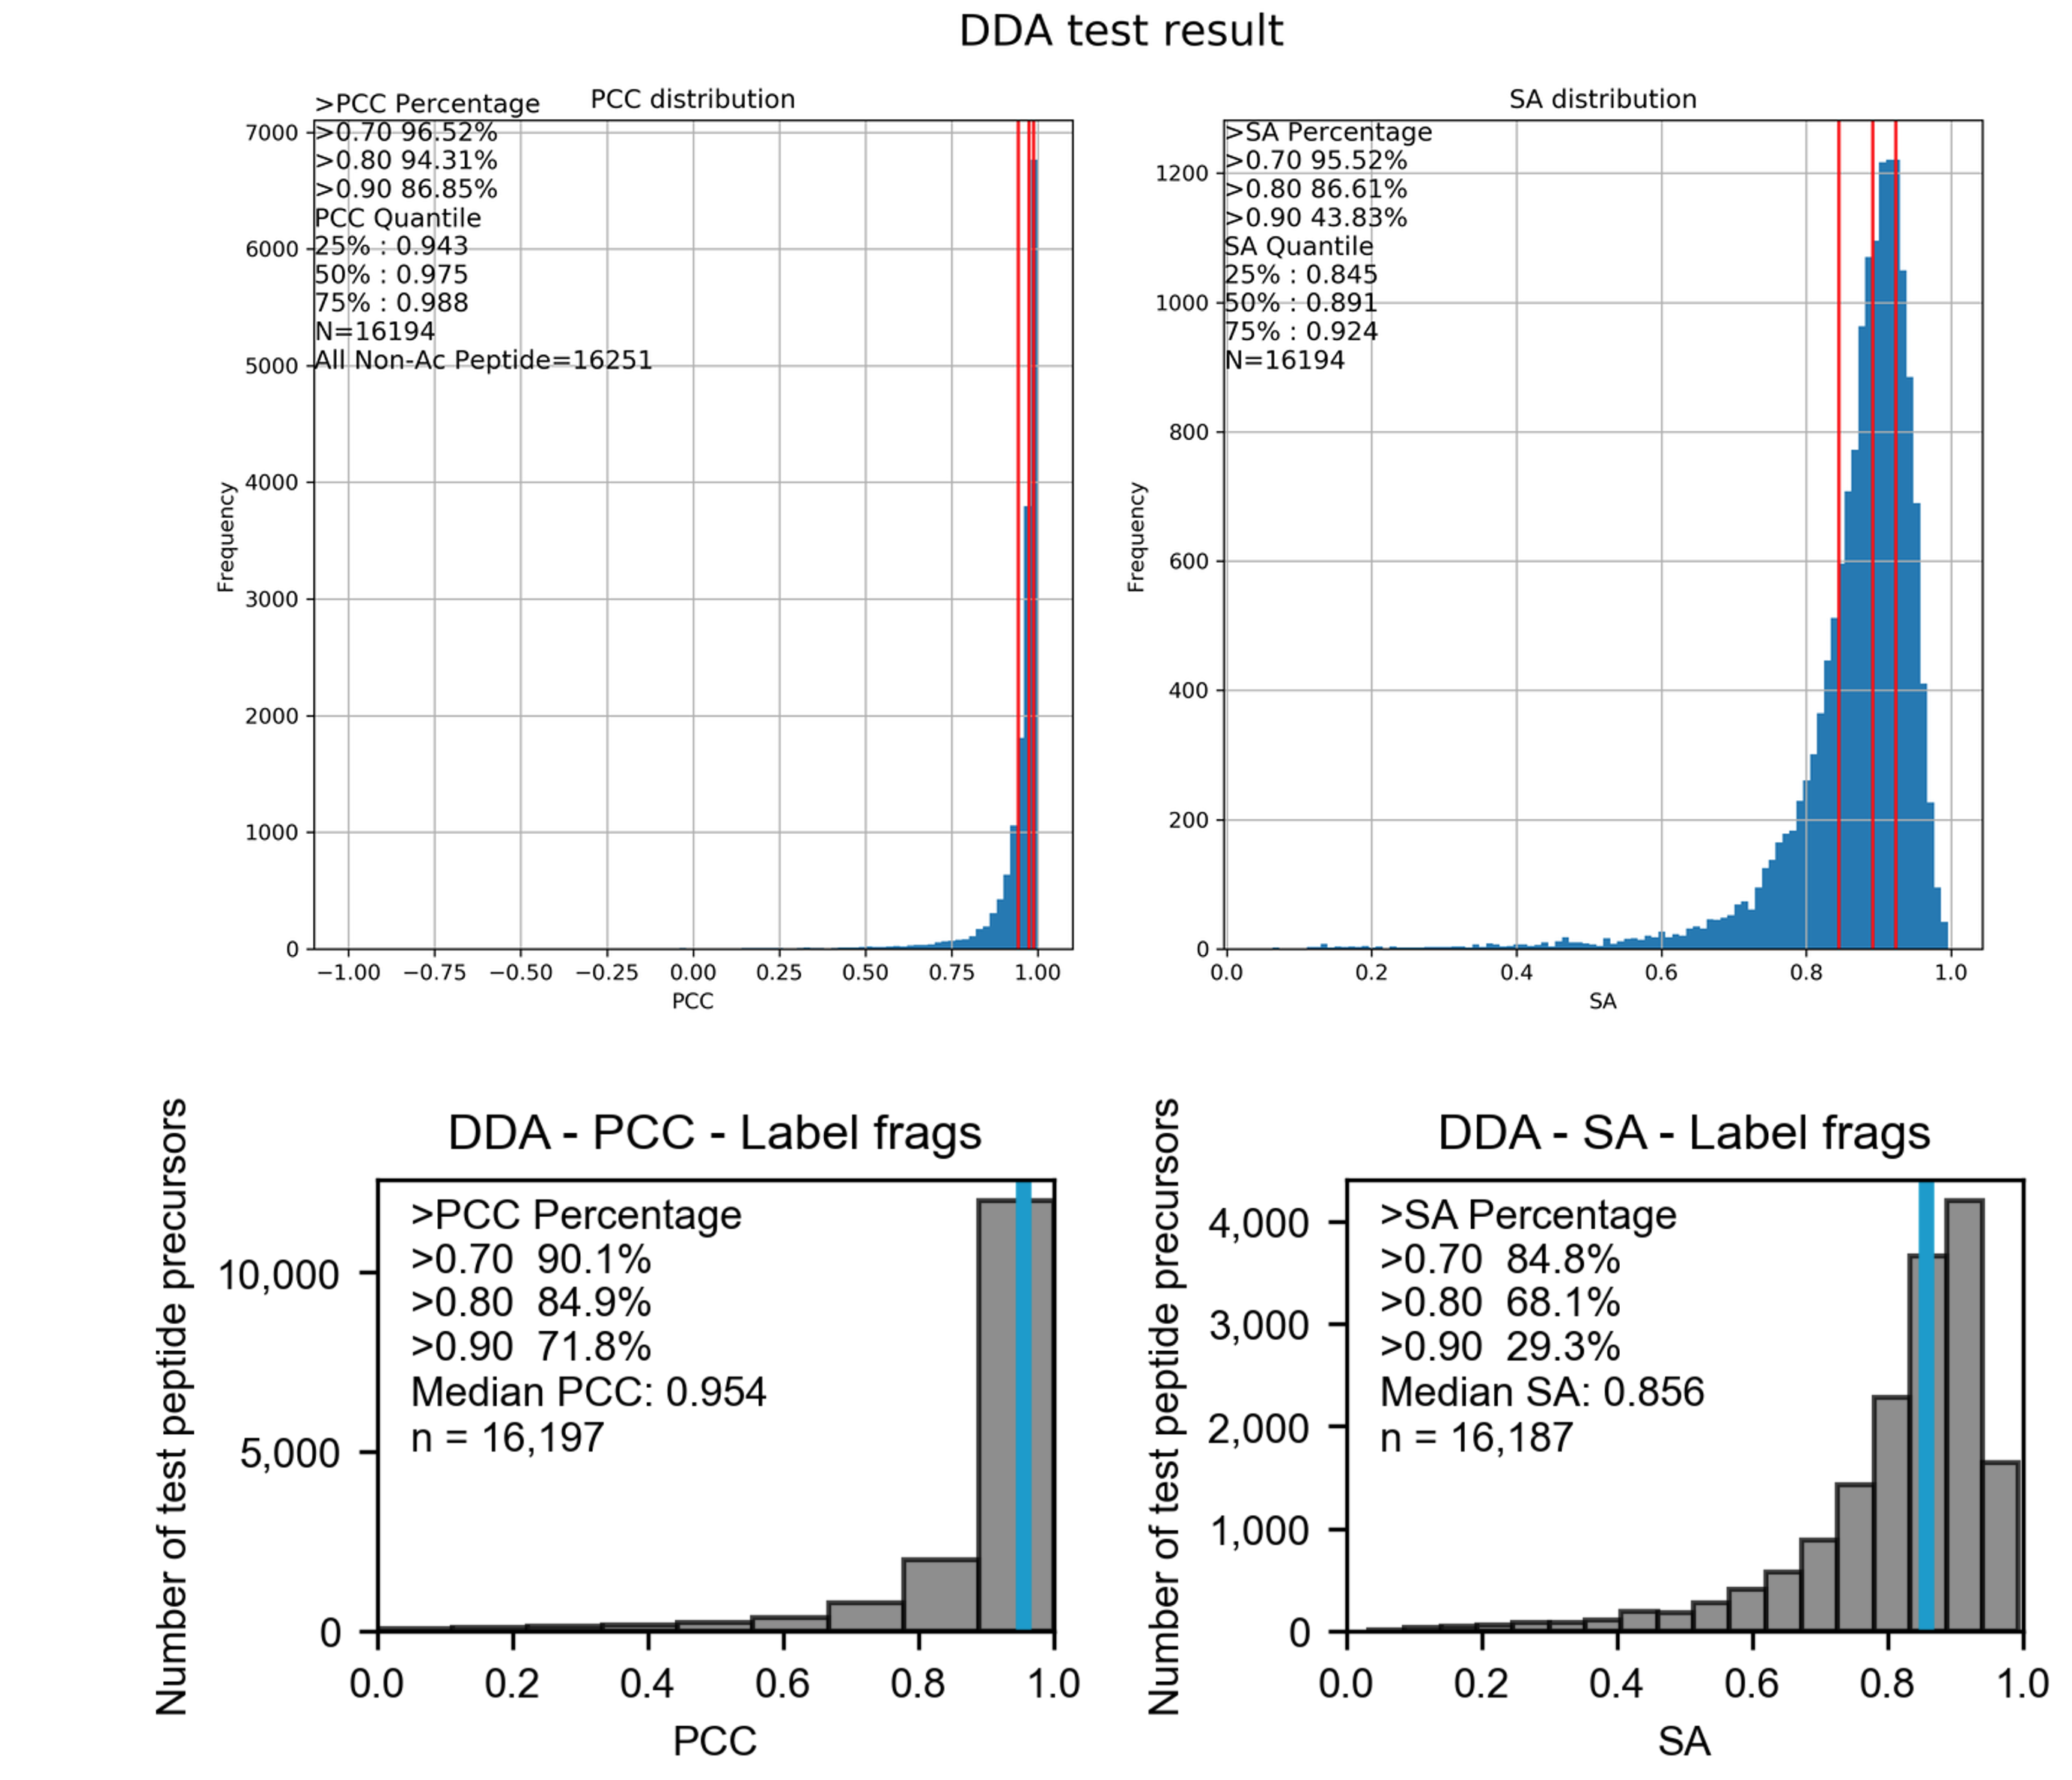
\includegraphics[width=3.0in]{DDA}
%
%   \caption{Visualization of performance of DDA dataset. The above is ours and the below is pdeep2}
%\label{fig:DDA}
%\end{figure}
%
%
%\begin{figure}[t]
%
%   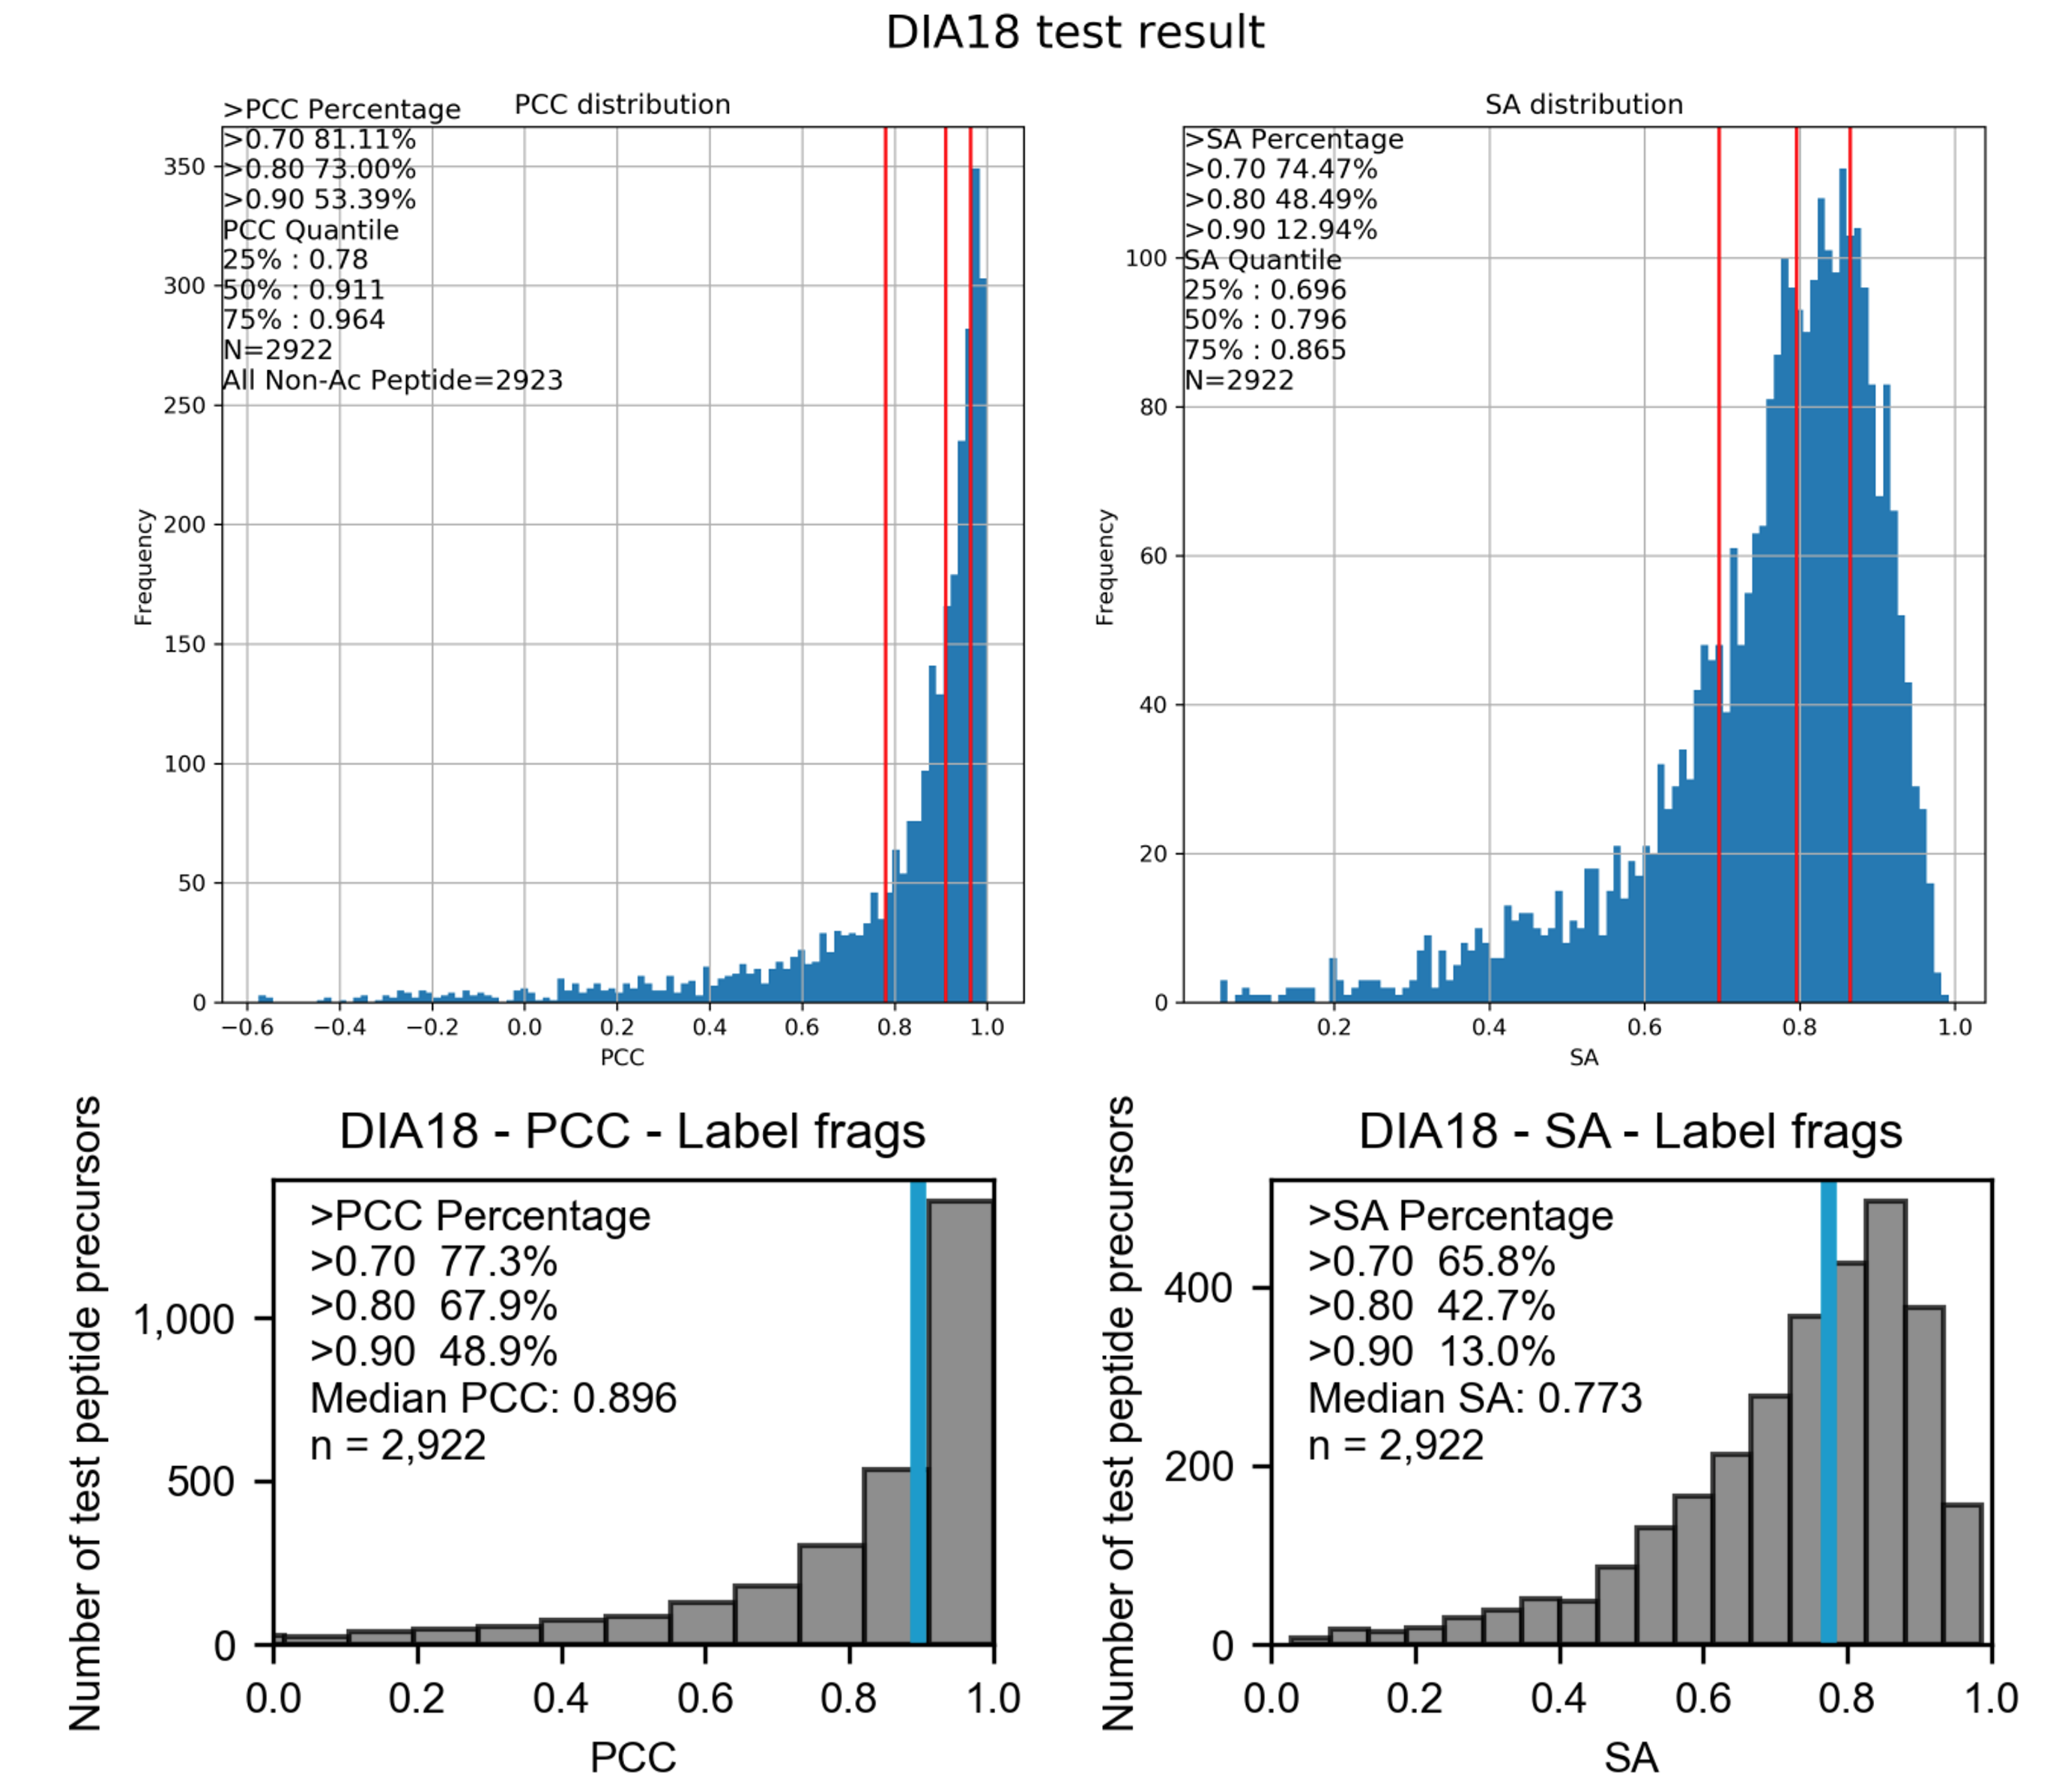
\includegraphics[width=3.0in]{DIA18}
%
%   \caption{Visualization of DIA18 dataset. The above is ours and the below is pdeep2}
%\label{fig:DIA18}
%\end{figure}
%
%
%\begin{figure}[t]
%
%   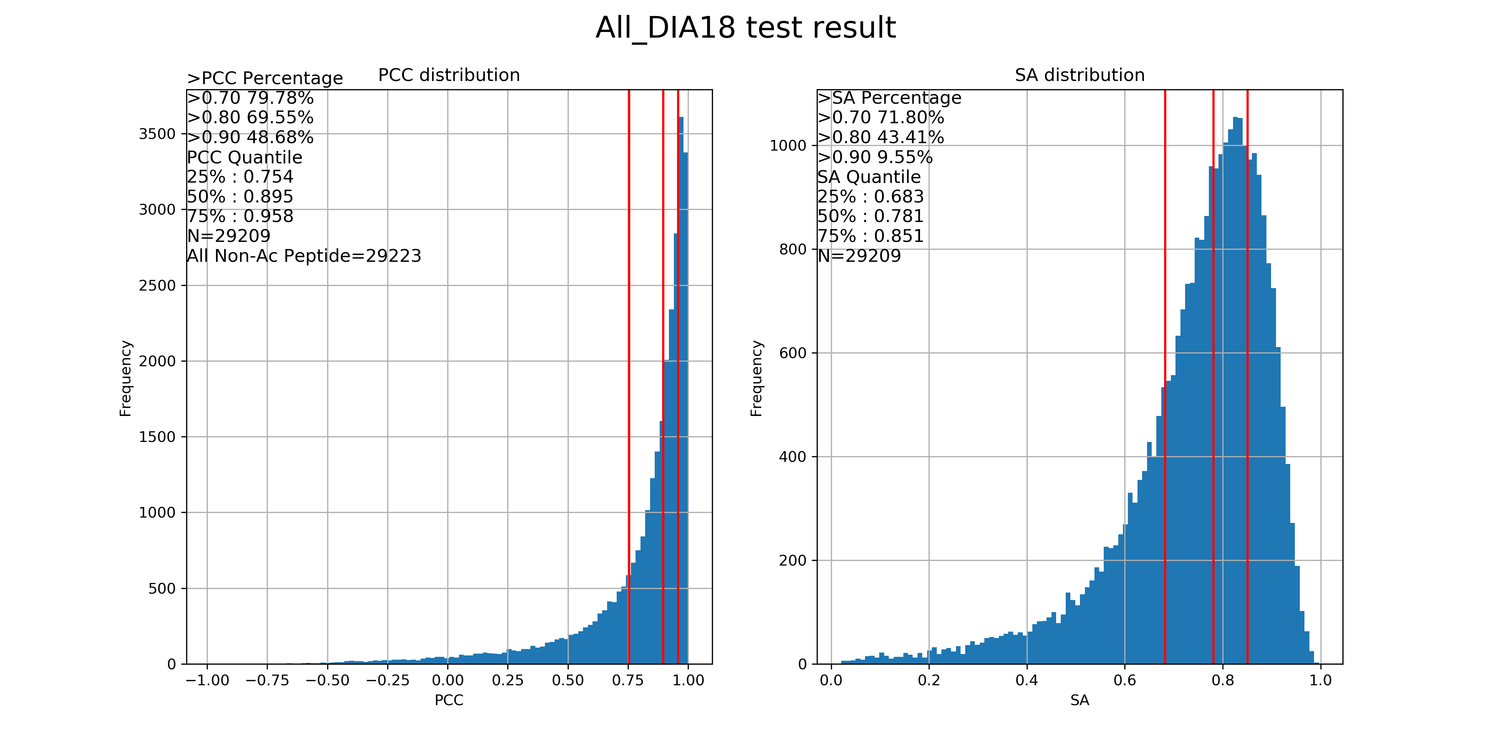
\includegraphics[width=3.5in]{DIA_direct_test}
%
%   \caption{Direct test on DIA18 dataset.}
%\label{fig:DIA18_direct}
%\end{figure}
%

\begin{table}
    \begin{center}
    \begin{tabularx}{\columnwidth}{|m{0.3\columnwidth}|Y|Y|}
    \hline
    data description & no. of peptides & no. of spectra\\
    \hline
    HumanPhosDB~\cite{lawrence2016plug} & 204,558 & -\\
    Jeff~\cite{liu2018vivo} & 67,552 & 89,437\\
    VeroE6~\cite{bouhaddou2020global} & 43,405  & 54,004\\
    R2P2~\cite{leutert2019r2} & 35,808 & 43,312\\
    U2OS-DIA~\cite{wang2020naguider} & 48,327 & 58,843\\
    RPE1-DIA~\cite{bekker2020rapid} & 33,576 & 39,977\\
    RPE1-DDA~\cite{bekker2020rapid} & 129,109 & 165,719\\
    \hline
    \end{tabularx}
    \end{center}
    \caption{Retention time datasets}
    \label{table:Datasets}
    \end{table}
 
    \begin{table}
       \begin{center}
      \resizebox{\columnwidth}{!}$ where the lower is the better, and the right is PCC where the higher is the better.}
       \label{table:Jeff}
       \end{table}
 
 \begin{table}
    \begin{center}
    \begin{tabular}{|l|c|c|}
    \hline
    Model & Median PCC & Median SA \\
    \hline\hline
    pdeep2 & 0.954 & 0.856 \\
    DeepPhospho$\star$ & 0.975 & 0.891 \\
    \hline
    \end{tabular}
    \end{center}
    \caption{DDA Dataset results.Ours is better.}
    \label{table:DDA}
    \end{table}
 
 \begin{table}
    \begin{center}
    \begin{tabular}{|l|c|c|}
    \hline
    Model & Median PCC & Median SA \\
    \hline\hline
    pdeep2 & 0.896 & 0.773 \\
    DeepPhospho$\star$ & 0.911 & 0.796 \\
    \hline
    \end{tabular}
    \end{center}
    \caption{DIA18 Dataset results.Ours is better.}
    \label{table:DIA18}
 \end{table}
 
 \begin{table}
    \begin{center}
    \begin{tabular}{|l|c|c|}
    \hline
    Model & Median PCC & Median SA \\
    \hline\hline
    Direct Test & 0.895 & 0.781 \\
    Train then Test & 0.911 & 0.796 \\
    \hline
    \end{tabular}
    \end{center}
    \caption{DIA18 Dataset results. Direct test only drops little compared to training and test}
    \label{table:DIA18_direct}
 \end{table}
 %%-------------------------------------------------------------------------